%%%%%%%%%%%%%%%%%%%%%
%   AMS packages    %
%%%%%%%%%%%%%%%%%%%%%
\documentclass{amsart}

\usepackage{amsmath}
\usepackage{amsxtra}
\usepackage{amscd}
\usepackage{amsthm}
\usepackage{amsfonts}
\usepackage{amssymb}
\usepackage{eucal}
\usepackage[all]{xy}
\usepackage{graphicx}
\usepackage{tikz-cd}
\usepackage{mathrsfs}
\usepackage{subfiles}
%\usepackage{mathpazo} not a huge fan
\usepackage{euler}
\usepackage{hyperref}
\usepackage{color}
\usepackage{longtable}
\usepackage{float}
\usepackage{caption}

\usepackage[colorinlistoftodos, textsize=tiny]{todonotes}
\def\listtodoname{List of Todos}
\def\listoftodos{\@starttoc{tdo}\listtodoname}

%\addtolength{\oddsidemargin}{-.5 in}
	%\addtolength{\evensidemargin}{-.4 in}
	%\addtolength{\textwidth}{1 in}
%
	%\addtolength{\topmargin}{0 in}
	%\addtolength{\textheight}{0 in}

\RequirePackage{color}
\definecolor{myred}{rgb}{0.75,0,0}
\definecolor{mygreen}{rgb}{0,0.5,0}
\definecolor{myblue}{rgb}{0,0,0.65}

%\usepackage{hyperref}
  %\hypersetup{colorlinks=true,citecolor=blue}

\usepackage{tikz}
\usepackage{tikz-cd}
\usetikzlibrary{matrix,arrows,decorations.pathmorphing}

%%%%%%%%%%%%%%%%%%%%%%% amsthm theorem styles %%%%%%%%
%%%%%%%%%%%%%%%

\theoremstyle{plain}
  \newtheorem{thm}{Theorem}[section]
  \newtheorem{prop}[thm]{Proposition}
  \newtheorem{lem}[thm]{Lemma}
  \newtheorem{cor}[thm]{Corollary}
	\newtheorem{claim}[thm]{Claim}
	\newtheorem{question}[thm]{Question}
	
\theoremstyle{definition}
  \newtheorem{defn}[thm]{Definition}
  \newtheorem{example}[thm]{Example}
  \newtheorem{exer}[thm]{Exercise}
  \newtheorem{ctexample}[thm]{Counterexample}
  \newtheorem{convention}[thm]{Convention}
	\newtheorem{conjecture}[thm]{Conjecture}
	
\theoremstyle{remark}
	\newtheorem{rem}[thm]{Remark}
  \newtheorem{note}[thm]{Notation}
  \newtheorem*{note*}{Notation}
  \newtheorem{case}{Case}
	
\numberwithin{equation}{section}

%%%%%%%%%%%%%%%%%%%%%%%%% custom commands %%%%%%%%%%%%%%%%%%%%%%%%%%%

\newcommand\nc{\newcommand}
\nc\on{\operatorname}
\nc\renc{\renewcommand}
\newcommand\ssec{\subsection}
\newcommand\sssec{\subsubsection}
\newcommand\bh{{\mathbb H}}
\newcommand\bn{{\mathbb N}}
\newcommand\bc{{\mathbb C}}
\newcommand\bbf{{\mathbb F}}
\newcommand\br{{\mathbb R}}
\newcommand\bq{{\mathbb Q}}
\newcommand\bp{{\mathbb P}}
\newcommand\bz{{\mathbb Z}}
\newcommand\ba{{\mathbb A}}
\newcommand\bk{{\Bbbk}}

\newcommand\sco{{\mathscr O}}

\newcommand{\id}{\mathrm{id}}
\newcommand\im{\text{im }}
\newcommand\coker{\text{coker}}
\newcommand\gal{\mathrm{Gal}}

\DeclareMathOperator{\ord}{ord}
\DeclareMathOperator{\sym}{Sym}

%%%%%%%%%%%%%%%%%%%%% cring custom commands %%%%%%%%%%%%%%%%%%%%%%%%%

\DeclareMathOperator\di{Div}
\newcommand\sx{\mathscr X}
\newcommand \subhalf[1]{\frac{{#1} - 1}{2{#1}}}
\newcommand{\se}[1]{\section*{Problem #1}}
\newcommand{\halfcan}{L}
\DeclareMathOperator{\supp}{Supp}
\DeclareMathOperator{\initial}{in_\prec}
\DeclareMathOperator{\gin}{gin}
\DeclareMathOperator{\Eff}{Eff}
\DeclareMathOperator{\sat}{sat}
\DeclareMathOperator{\newspan}{span}
\DeclareMathOperator{\proj}{Proj}
\DeclareMathOperator{\spec}{Spec}
%\captionsetup[table]{belowskip = 4pt}

\makeatletter
\newcommand{\customlabel}[2]{%
   \protected@write \@auxout {}{\string \newlabel {#1}{{#2}{\thepage}{#2}{#1}{}} }%
   \hypertarget{#1}{#2}
}
\makeatother

%%%%%%%%%%%%%%%%%%%%%%%%%%%%%% title %%%%%%%%%%%%%%%%%%%%%%%%%%%%%%%%

\title{Canonical rings of rational divisors on projective space and Hirzebruch surfaces}

\author{Aaron Landesman}
\address[Aaron Landesman]{Department of Mathematics, Harvard University}
\email{aaronlandesman@college.harvard.edu}

\author{Peter Ruhm}
\address[Peter Ruhm]{Department of Mathematics, Stanford University}
\email{pruhm@stanford.edu}

\author{Robin Zhang}
\address[Robin Zhang]{Department of Mathematics, Stanford University}
\email{robinz16@stanford.edu}

\date{\today}

%%%%%%%%%%%%%%%%%%%%%%%%%%%%% document %%%%%%%%%%%%%%%%%%%%%%%%%%%%%%

\begin{document}

\begin{abstract}
 	Bounding generator and relation degrees of general $\bq$-divisors
	on projective spaces $\bp^n$ and Hirzebruch surfaces.
\end{abstract}

\maketitle

%%%%%%%%%%%%%%%%%%%%%%%%%%%% Introduction %%%%%%%%%%%%%%%%%%%%%%%%%%%%%%%

\section{Introduction}

\section{Background}

\begin{defn}
\label{defn:lower-approximation}
If $\frac{\alpha}{\beta}\in \bq$, then $\frac{c}{k}$ (written in
reduced form with $c \in \bn, k \in \bn$) is a {\bf{best lower
approximation}} to $\frac{\alpha}{\beta}$ if there does not exist
any $\frac{c'}{k'}\in \bq$ with $0 < k'<k$ and $\frac{c}{k} \le
\frac{c'}{k'}$.
\end{defn}

Moreover, if $\frac{\alpha}{\beta}\ge 0$, then the non-negative
best lower approximations of $\frac{\alpha}{\beta}$ form a finite
sequence
\[
	0 = \frac{c_0}{k_0} < \frac{c_1}{k_1} < \ldots < \frac{c_r}{k_r} = \frac{\alpha}{\beta}.
\]
Figure \ref{fig:s14/5-lattice} gives a pictorial representation of
the positive best lower approximations of $\frac{\alpha}{\beta} =
\frac{14}{5}$.

\begin{figure}
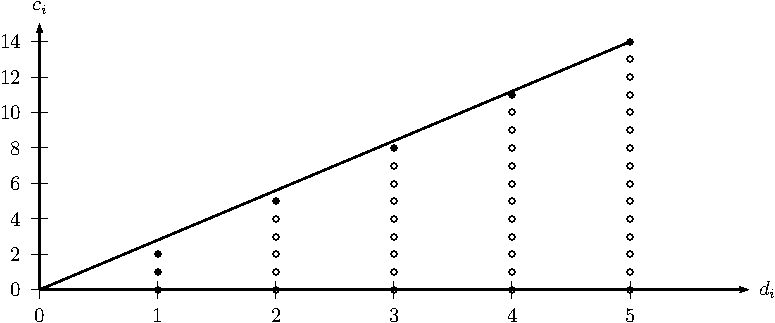
\includegraphics{pics/spin-lower-approximations-pic-pics.pdf}
\caption{This figure shows each non-negative best lower
approximation of $\frac{14}{5}.$ Each ``$\bullet$'' denotes a best
lower approximation and each ``$\circ$'' denotes a lattice point
below $5y=14x$ which is not a best lower approximation.  Note that
the non-negative best lower approximations generate the monoid of
lattice points in the first quadrant satisfying  $5y \le 14x$, with
the operation $(a_1, b_1)(a_2, b_2)\mapsto (a_1 + a_2, b_1 + b_2)$.}
\label{fig:s14/5-lattice}
\end{figure}

\ssec{Notation}
\begin{convention}
Write
\begin{align*}
	D = \sum_{i=1}^{n}\alpha_i D_i.
\end{align*}
where $\alpha_i \in \bq$.
\end{convention}

\begin{convention}
Let $\{x_0, \ldots, x_m\}$ be coordinates for $\bp^m$. Let
$\vec{v} = (v_0, \ldots, v_m) \in \br^{m + 1}$. Then write
\[
	x_{\vec{v}} := \prod_{i = 0}^{m} x_i^{v_i}
\]
\end{convention}

\section{Lemmas for Generation and Relations}

\begin{prop}
\label{prop:cone-generation}
Let $n,t \in \bz,$ let $\alpha_1, \ldots, \alpha_n \in \bq$ and let $k_i^j \in \bz$ with $1 \leq i \leq n, 1 \leq j \leq t.$ Define
\begin{align*}
	\Sigma = \{(d,c_1, \ldots, c_n) \in \bz^{n+1} : c_i \geq - d \alpha_i,1 \leq i \leq n \text{ and } \sum_{i=1}^{n}k_i^j = 0, 1 \leq j \leq t\}
\end{align*}
Let $e_1, \ldots, e_r \in \Sigma,$ with $e_i = (\delta^i, c_1^i, \ldots, c_n^i)$ be a set of {\bf extremal rays} of $\Sigma$, meaning that the $\Sigma$ is contained in the $R_{\geq 0}$ span of $e_1, \ldots, e_r$.  Then, as a semigroup, $\Sigma$ is generated by elements whose first coordinate is less than $\sum_{i=1}^{n}\delta_i$. Furthermore, every element $\sigma \in \Sigma$ can be written in a canonical form $\lambda + \sum_{i=1}^{r} w_i e_i,$ with the first coordinate of $\lambda$ less than $\sum_{i=1}^{r}\delta_i$ and $w_1,\ldots, w_r \in \bz$.
\end{prop}
\begin{proof}
By assumption, $\sigma \in \Sigma$ as $\sigma = \sum_{i=1}^{r}a_i e_i$ with $a_i \in \br$. Let $\{a\} := a - \lfloor a \rfloor$ denote the fractional part of $a$. Let $\lambda = \sum_{i=1}^{r}\{a_i\}$. Hence, we can write $\sigma = \lambda + \sum_{i=1}^{r}\lfloor a_i \rfloor e_i.$ Hence, $\sigma$ lies in the $\bz_{\geq 0}$ span of $\lambda, e_1,\ldots, e_r$, which all have first coordinate less than $\sum_{i=1}^{r}\delta_i$. Therefore, $\Sigma$ is generated by elements whose first coordinate is less than $\sum_{i=1}^{r}\delta_i$.
\end{proof}

\begin{lem}
\label{lem:composite-map}
Let $D = \sum_{i=1}^{n}\alpha_i D_i$ where $D_i = V(f_i)$. Suppose we have a surjection $\phi: \bk[x_1,x_2,\ldots, x_r] \rightarrow R_D, x_i \mapsto p_i(f_1, \ldots, f_n),$ where $p_i$ is a monomial in $f_1,\ldots, f_n$. Then, define
\begin{align*}
	\Sigma = \langle u^d y_1^{c_1} \cdots y_n^{c_n} : c_i \geq -d \alpha_i, \sum_{i=1}^{n}a_ic_i = \sum_{i=1}^{} b_i c_i. \rangle 
\end{align*}
In this case, we have a factorization of $\phi$ given by maps $\chi, \psi$ defined by
\todo{Make this have mapsto on bottom}
$$\begin{tikzcd}
\bk[x_1,\ldots, x_r] \ar {r}{\chi} & \bk[\Sigma] \ar {r}{\psi} & R_D \\
x_i \ar r & u^{d_i}y_1^{c_{i1}} \cdots y_n^{c_{in}} \ar r & u^{d_i}f_1^{c_{i1}} \cdots f_n^{c_{in}}
\end{tikzcd}$$
Assuming $\chi$ is surjective, the minimal degree of generation of $\ker \phi$ is at most the maximum of the minimal degree of generation of $\ker \chi$ and the minimal degree of generation of $\ker \psi$.
\end{lem}
\begin{proof}
Note that we have an exact sequence
$$\begin{tikzcd}
0 \ar r & \ker \chi \ar r & \ker \phi \ar r & \ker \psi \ar r & 0
\end{tikzcd}.$$
To see this, note that the left map is an inclusion because $\phi = \chi \circ \psi$. Next, the right map, given by $\chi|_{\ker \phi}:\ker \phi \rightarrow \ker \psi$ is a surjection, again because $\phi = \chi \circ \psi$. The composition of the two maps is $0$ by definition of the kernel of $\chi$. Finally, if $a \in \ker \phi$ and $a$ lies in the kernel of the right map, then by definition $\chi(a) = 0$.
\end{proof}

\begin{lem}
\label{lem:bound-ker-chi}
Retaining the notation of Lemma ~\ref{lem:composite-map}, if $\Sigma$ has extremal rays $e_1,\ldots, e_r$ in degrees $d_1, \ldots, d_r$ then $\ker \chi$ has a system of generators in degrees less than $\sum_{i=1}^{r}d_r-1$.
\end{lem}
\begin{proof}
Since $e_1, \ldots, e_r$ are extremal rays, by Proposition ~\ref{prop:cone-generation}, every element $\sigma \in \Sigma$ can be written in a canonical form $\lambda + \sum_{i=1}^{r}e_i$. Now, letting $\lambda_0 := 0,\lambda_1, \ldots, \lambda_m$ be all elements of $\Sigma$ so that we can write $\lambda_i = \sum_{i=1}^{r}a_i e_i$ with $0 \leq a_i < 1$ for all $i$. Then, for any $1 \leq i \leq j \leq m,$ we can write $\lambda_i + \lambda_j$ in the above canonical form, yielding a relation in degree at most $\deg \lambda_i + \deg \lambda_j \leq 2 \cdot \left( \sum_{i=1}^{r}d_r -1 \right).$ Furthermore, these relations generate all relations, as one can apply a sequence of these relations to put any $\sigma \in \Sigma$ into canonical form.
\end{proof}


\section{Canonical Rings on Projective Space}
In this section, we bound the degrees of generators and relations for divisors on $\bp^m$, for all $m \geq 1$. The $n = 1$ case was covered in \cite{dorney:canonical}.

\ssec{Preliminaries on Projective Space}

For the remainder of this section, we shall fix $m \geq 1$ and choose an isomorphism $\bp^m \cong \proj V$ so that $x_0,\ldots, x_m$ form a basis for $V$. Through the rest of this section, we will think of $x_i$ as a rational section of $H^0(\bp^m, \sco_{\bp^m})$ of degree 1.


Write
\begin{align*}
	D = \sum_{i=0}^{n}\alpha_i D_i.
\end{align*}
where $\alpha_i \in \bq$ and $\deg D_i = a_i$. Let $f_i$ be Cartier divisors such that $D_i = V(f_i)$. We shall further assume that among there exist functions $f_0,\ldots, f_{m+1}$ form a basis for degree one rational functions on $\bp^m$.

\todo{possibly change this to only have two equations}
\begin{prop}
\label{prop:pm-span-and-basis}
The functions $u^d \cdot \prod_{i=1}^n f_i^{c_i}$ so that 
\begin{align}
\label{align:pm-span}
\sum_{i=0}^{n} c_i \cdot a_i \cdot f_i = 0 & \text{ and } &c_i \geq \lfloor \alpha_i d\rfloor	
\end{align}
form a spanning set for $H^0(\bp^m, dD)$ over $k$. Furthermore, functions 
of the form $u^d \cdot \prod_{i=1}^n f_i^{c_i} $ such that
\begin{align}
\label{align:pm-basis}
c_i = -\lfloor d\alpha_i \rfloor & \text{ for } & i > m
\end{align}
form a basis for $H^0(\bp^m, dD)$ over $k$.
\end{prop}
\begin{proof}
By definition of $H^0(\bp^m,dD)$, functions satisfying conditions 
~\eqref{align:pm-span} lie in $H^0(\bp^m,dD)$. To complete the proof, it suffices to check functions satisfying conditions ~\eqref{align:pm-basis} form a basis of $H^0(\bp^m,dD)$. Note that there $\binom{m+ \lfloor dD \rfloor }{m}$ functions satisfying condition ~\eqref{align:pm-basis}. However we know $h^0(\bp^m,dD) = \binom{m+ \lfloor dD \rfloor }{m},$ so it suffices to show that those functions satisfying condition ~\eqref{align:pm-basis} are independent. This follows from the assumption that $f_0,\ldots, f_n$ form a basis of degree 1 rational functions, and so degree $\lfloor d \deg D \rfloor $ monomials in $f_0,\ldots, f_n$ form a basis of degree $\lfloor d \deg D \rfloor $ rational functions.
\end{proof}
\todo{the following bound is the generation bound beginning from evan's paper}


\ssec{One point on Projective Space}
\label{ssec:proj-one-point}

\begin{rem}
Remark about how we can assume divisor only consists of hyperplanes
by taking the Veronese embedding.
\todo{write}
\end{rem}


\begin{thm}
\label{thm:proj-one-point}
Let $X = \bp^m$ with $\{x_0, \ldots, x_m\}$ a coordinate system for
$\bp^m$. Let $D = \alpha H$, with $\alpha = \frac{a}{b} \in \bq$
and $H = V(x_k)$ a hyperplane of $\bp^m$, be a divisor on $\bp^m$.
Let
\[
	\left\lfloor \frac{a}{b} \right\rfloor = \frac{c_0}{d_0} <
	\frac{c_1}{d_1} < \ldots < \frac{c_r}{d_r} = \frac{a}{b}
\]

\noindent
be the best lower approximations of $\alpha$. Then the
canonical ring
\[
	R_D := \bigoplus_{d \geq 0} H^0(\bp^m, \lfloor dD \rfloor)
\]

\noindent
has a minimal presentation consisting of the $\sum_{i = 0}^{r}
{{m + i} \choose {i}}$ generators $f_{\vec{v}} := \frac{u^{a_i}
x^{\vec{v}}}{x_k^{c_i}}$ where $\vec{v} \in \bz_{\geq 0}^{m + 1}$
such that $\sum_{j = 0}^{m} v_j = c_i$ and $z$ \todo{how many?}
relations of the form
\[
	f_{d_i}^{\vec{v}} f_{d_j}^{\vec{w}} = f_{d_k}^{\vec{y}} f_{d_\ell}^{\vec{z}}
\]

\noindent
when $d_i + d_j = d_k + d_\ell$ and $\vec{v} + \vec{w} = \vec{y} +
\vec{z}$.
\end{thm}

\begin{proof}
We know $\{f_{0}^{\vec{v}} : \deg \vec{v} = \left\lfloor \frac{a}{b}
\right\rfloor \}$ are minimal generators in degree $1$. Now let $i >
0$. If $f_{d_i}^{\vec{v}}$ were not minimal for some $\vec{v}$ such
that $\deg \vec{v} = c_i$, then $f_{d_i}^{\vec{v}} = f_{s}^{\vec{w}}
f_{t}^{\vec{z}}$ for some $s, t \in \bn$ and $\vec{w}, \vec{z} \in
\bz_{\geq 0}^{m + 1}$. In particular, we see that 
\begin{align*}
	&d_i = s + t \\
	&c_i = \deg \vec{v} = \deg \vec{w} + \deg \vec{z}
\end{align*}

\noindent
so $\frac{c_i}{d_i}$ is the mediant of the rational numbers
$\frac{\deg \vec{w}}{s}, \frac{\deg \vec{z}}{t}$ which both
do not exceed $\alpha$. One of $\frac{\deg \vec{w}}{s},
\frac{\deg \vec{z}}{t}$ must be at least $\frac{c_i}{d_i}$
and $s$ and $t$ are both less than $d_i$, so we have a contradiction 
of $\frac{c_i}{d_i}$ being a best lower approximation of $\alpha$
(see Definition ~\ref{defn:lower-approximation}).

Now we show that no further generators are necessary. As done in
the proof of the $\bp^1$ case by O'Dorney \cite[Theorem 6]
{dorney:canonical}, each lattice point $(d, c) \in \bz_{\geq 0}^2$
such that $c \leq d \alpha$ is a nonnegative linear combination of
$\vec{x}_i$ and $\vec{x}_{i + 1}$ where $\vec{x}_i := (d_i, c_i) \in
\bz^2$. Consequently, any element $\frac{u^{d} x^{\vec{v}}}
{x_k^{c}} \in R_D$ is expressible as
\begin{align*}
	\frac{u^{d} x^{\vec{v}}} {x_k^{c}} = \frac{u^{d_i} x^{\vec{w}}}
	{x_k^{c_i}} \frac{u^{d_{i + 1}} x^{\vec{z}}} {x_k^{c_{i + 1}}}
\end{align*}

\noindent
where $\vec{w}, \vec{z} \in \bz_{\geq 0}^{m + 1}$ such that $\deg
\vec{w} = c_i, \deg \vec{z} = c_{i + 1}$. But these are precisely
two generators of the form $f_{d_i}^{\vec{w}}$ and $f_{d_{i + 1}}
^{\vec{z}}$ as prescribed in the theorem statement.

\todo{relations}
\end{proof}



\ssec{Bounds for Arbitrary Divisors on Projective Space}

\begin{rem}
When $\langle f_1, \ldots, f_r \rangle = \langle x_0, \ldots, x_n \rangle$ (the irrelevant ideal), we may directly use the hypersurface method by considering $x_0, \ldots, x_n$ instead of the $f_i$'s. However, when $\sqrt{\langle f_1, \ldots, f_r \rangle} = \langle x_0, \ldots, x_n \rangle$ (or the saturation), we cannot obtain the same result from our modification of O'Dorney's method as seen in Example ~\ref{eg:radical}. Instead we must use ghost points and hypersurfaces.
\end{rem}

\begin{example}
\label{eg:radical}
As an example for why we need to add in ghost points for $\bp^2$, consider $\frac{-1}{5}V(x_0^2) + \frac{1}{7}V(x_1^2) + \frac{1}{17}V(x_2^2)$. In degree $595 = 5* 7 * 17$, this has dimension $6$, but we cannot possibly use the lattice approach, as all lower degrees only have dimension 1. In fact, we may construct similar examples using any $x_i^m$ for $f_i$ with appropriate coefficients.
\end{example}
\todo{construct class of additional examples}
\todo{The example above needs to be changed because $x_0^2$ can be replaced by $2x_0$}

\section{Canonical Rings on Hirzebruch surfaces}
Let $D=\sum_{i=1}^m \alpha_i C_i$ for some curve $C_i\in F_k$, such
that $C_1, \ldots, C_4$ are independent curves with bi-degrees $(1,0)
, (1,0), (0,1)$, and $(0,1)$ respectively. Let $C_i = V(f_i)$ where
$f_i \in \mathscr{O}(a_i, b_i)$. Then each $C_i$ corresponds to a
polynomial $f_i$ where $f_1$ and $f_2$ are independent linear
polynomials in $x_0$ and $x_1$ and $f_3$ and $f_4$ are independent
linear polynomials in $y_0$ and $y_1$.

\begin{defn}
Suppose $D = \sum_{i=1}^m \alpha_i C_i \in \mathbb{Q} \otimes \di(F_
k)$. Then define 
\begin{equation}\label{eqn:define-T=(D)}
	T_=(D) = \left\{i \in \{1, \ldots, m\}: a_i \sum_{k=1}^m b_k 
\alpha_k = b_i \sum_{k=1}^m a_k \alpha_k \right\},
\end{equation}

\begin{equation}\label{eqn:define-T+(D)}
	T_+(D) = \left\{ i \in \{1, \ldots, m\}:  \vphantom{\sum_{k=1}^m} 
a_i \sum_{k=1}^m \alpha_k b_k > b_i \sum_{k=1}^m \alpha_k a_k 
\right\},
\end{equation}

\noindent
and
\begin{equation}\label{eqn:define-T-(D)}
	T_-(D) = \left\{ j \in \{1, \ldots, m\}: a_j \sum_{k=1}^m \alpha_
k b_k < b_j \sum_{k=1}^m \alpha_k a_k s \right\}.
\end{equation}
\end{defn}

\begin{lem}
$R_D$ is generated in degree at most
\[
	\sum_{i\in T_=(D)} \gcd(a_i, b_i)\ell_i + \sum_{i\in T_+(D) \atop j\in T_-(D)} (a_i b_j- a_j b_i)\ell_{i,j}.
\]
\end{lem}

\begin{proof}
Let $(a_i, b_i)$ be the bi-degrees of $f_i$. Notice that if $\gamma
\in (R_D)_d$, then 
\[
	g = \sum_{i=1}^m {f_i}^{c_i}
\]

\noindent
where each $c_i \ge - \alpha_i c_i$, $\sum_{i=1}^m c_i a_i = 0$,
and $\sum_{i=1}^m c_i b_i = 0$. Then we can view $g$ inside of the
lattice $S \subseteq \mathbb{R}^{n + 1}$ given by ordered elements of
the form $(d, c_1, \ldots, c_n)$ satisfying $c_i \ge - d \alpha_i$
for all $i$, $\sum_{i=1}^m c_i a_i = 0$, and $\sum_{i = 1}^m c_i b_i =
 0$. From here, determining a spanning set for $(R_D)_d$ reduces to
finding the extremal rays of $S$ \todo{cite previous lemma}.

To do this, we extend the method of O'Dorney \todo{cite}. We first
view the cone inside of $\mathbb{R}^{n+1}$ given by elements of the
form $(d, c_1, \ldots, c_n)$ satisfying $c_i \ge -\alpha_i d$ for
all $i$ and $\sum_{i = 1}^n c_i (a_i + b_i) =0$. By O'Dorney, this
has extremal rays given by
 
\[
	e_i = (1, -\alpha_1, \ldots, -\alpha_{i-1}, \frac{\sum_{j \ne i}
	\alpha_j(a_j+ b_j)}{a_i + b_i}, -\alpha_{i + 1}, \ldots, - \alpha_m).
\]

Let $\Delta^{n-1}$ be the simplex with vertices $e_1, \ldots e_m$.
We can then intersect the hyperplane $H$ given $\sum_{i=1}^m a_i X_i
= 0$ to get a subspace $S$. The extremal rays of $S$ are given
by the set of $e_i$ contained in $H$ together with the points of
intersection $e_{i,j}$ of $H$ and the line segment connecting $e_i,
e_j \not \in H$.

We can calculate the following elements of $R_D$ whose
corresponding lattice points lie on these extremal rays:

For $i \in T_=(D)$
define
\[
	\epsilon_i := (\prod_{k \ne i} f_k^{-\alpha \ell_i \gcd(a_i, b_i)})
	(f_i^{\ell_i \frac{\gcd(a_i, b_i)}{a_i + b_i}\sum_{k \ne i}
	\alpha_k (a_k + b_k)}) \in H^0(\ell_i \gcd(a_i, b_i) D).
\]

For $i \in T_+(D)$ and $j \in T_-(D)$, define
\[
	\epsilon_{i, j} := (\prod_{k = 1}^m f_k^{-\alpha \ell_{i,j} (a_i b_
j - a_j b_i)}) {f_i}^{s_1} {f_j}^{s_2} \in H^0(\ell_{i,j}(a_i b_j - 
a_j b_i)D)
\]

where
\[
	s_1 = b_j \sum_{k \ne i,j} \alpha_k a_k - a_j \sum_{k\ne i, j}
	\alpha_k b_k
\]

\noindent
and
\[
	s_2 = b_i \sum_{k \ne i,j} \alpha_k a_k - a_i \sum_{k \ne i, j}
	\alpha_k b_k.
\]

Let $E$ be the set of $\epsilon_i$ and $\epsilon_{i,j}$ given 
above, satisfying the respective conditions.
$E$ satisfies the conditions of proposition \todo{cite earlier 
proposition}, so by applying that proposition $R_D$ is generated in 
degree at most
\[
	\sum_{i\in T_=(D)} \gcd(a_i, b_i)\ell_i + \sum_{i\in T_+(D) \atop
	j \in T_-(D)} (a_i b_j- a_j b_i)\ell_{i,j}.
\]
\end{proof}

\todo{factor $\phi$ through $\psi$ and $\chi$.}
\begin{lem}
$\ker(\psi)$ is generated in degree at most \todo{insert number}.
\end{lem}

\begin{proof}
We first claim that $\psi$ has a relation of the form
\begin{equation}\label{eqn:relations-psi}
	(y_j - \beta_j)\prod_{i=1}^m {y_i}^{c_{i}}
\end{equation}

\noindent
for some $d\in \mathbb{N}$, $c_i \ge -\alpha_i d$, $a_j + \sum_{i = 1}
^m a_i c_i = 0$, $b_j + \sum_{i=1}^m b_i c_i = 0$, and $\beta_j \in
k[y_1, \ldots, y_4]$ satisfies $\psi(\beta_j)\in \mathscr{O}(a_j,
b_j)$.

To find such a $\beta$, we simply write $\epsilon_j$ as a 
polynomial in $\epsilon_1, \ldots \epsilon _4$. Furthermore, these
generate all relations, since they allow us to reduce any $\prod_{i =
1}^n \epsilon_i^{r_i}$ to a canonical form. \todo{add reference to
earlier description of canonical form.}

Note that we can view the relations from Equation
\ref{eqn:relations-psi} as an element of $\mathbb{R}^{n+1}$ given
by $(d, c_1, \ldots, c_n)$.  Let $S'\subseteq \mathbb{R}^{+}$ be the
set of $(d, c_1, \ldots, c_n)$ satisfying $c_i \ge -\alpha_i d$,
$a_j + \sum_{i = 1}^m a_i c_i = 0$, and $b_j + \sum_{i=1}^m b_i c_i
= 0$.  Note that $S'$ is a translation of $S$ by \todo{finish}

\end{proof}


%%%%%%%%%%%%%%%%%%%%%%%%% Acknowledgements %%%%%%%%%%%%%%%%%%%%%%%%%%%%

\section{Acknowledgments}
We are grateful to David Zureick-Brown for introducing us to this
subject, for providing invaluable guidance,
and for his mentorship. We also thank Ken Ono and the
Emory University Number Theory REU for arranging our project and
providing a great environment for mathematical learning and
collaboration.
Finally, we gratefully acknowledge the financial support given by
NSF Grant Award Number 1250467 via the Emory University Number
Theory REU. We deeply appreciate all of the support that has made
our work possible.

%%%%%%%%%%%%%%%%%%%%%%%%%%%% References %%%%%%%%%%%%%%%%%%%%%%%%%%%%%%%

\nocite{*}
\bibliography{bibliography-stacky-surface}{}
\bibliographystyle{plain}

\end{document}